\documentclass[a4paper,natbib,man]{apa6}

\usepackage[english]{babel}
\usepackage[utf8x]{inputenc}
\usepackage{amsmath}
\usepackage{graphicx}
\usepackage{soul}

\title{The economics and timing of active word learning (WORKING TITLE / DRAFT SKELETON)}
\shorttitle{Economics of active word learning}
\author{Shohei Hidaka$^1$, Takuma Torii$^1$, and George Kachergis$^2$}
\affiliation{$^1$School of Knowledge Science, Japan Advanced Institute of Science and Technology, Nomi, Ishikawa, 923-1292, Japan and $^2$Department of Psychology, Stanford University, Stanford, CA, 94305, USA}

\begin{document}
\maketitle

% ============================================================================
% NOTE (not for submission): this file was split off from
% paper/main_revised.tex (the "Active learning expedites cross-situational
% word learning" paper). That paper establishes that active selection of
% learning situations dramatically speeds up word learning under Zipfian
% distributions, robustly across idealized analysis, incremental simulation,
% and real data (SUN, Flickr8k). This draft assumes that result and asks a
% different, narrower question: given that active selection helps, how
% should a resource- or time-constrained learner actually deploy it? The two
% sections below were originally written as Appendix F (linger-vs-move-on on
% real Flickr8k captions) and Appendix G (a developmental passive-to-active
% trajectory) of that paper; they are reproduced here essentially verbatim,
% since both are self-contained, complete results, not stubs. What's missing
% is everything that makes this its own paper: an Introduction motivating
% the shared question, a Discussion connecting the two results to each
% other and to the literature, and probably additional evidence (the
% Introduction bullets below sketch what that might look like).
% ============================================================================

\section{Introduction (bullet-point sketch, not prose)}

\begin{itemize}
\item \textbf{The starting point.} Hidaka, Torii, \& Kachergis (companion paper) show that active selection of learning situations--choosing which word to target, and/or which distractors accompany it--dramatically speeds up cross-situational word learning under Zipfian word and referent distributions, robustly across idealized analysis, incremental simulation with three distinct learning mechanisms, and two independent real datasets (SUN scene database, Flickr8k captions).

\item \textbf{The gap that paper leaves open.} Throughout, ``active'' is treated as a fixed, idealized property of the learner: active on every episode or on none, for the whole simulated run, and when active, free to choose among the entire vocabulary. Three things this abstraction leaves out:
  \begin{itemize}
  \item[--] \textit{Situations aren't free to obtain, and not all ways of obtaining one cost the same.} Real active selection isn't just ``pick a target word''--a learner (or caregiver) can also choose whether to linger on the situation already in front of them (ask for more information about the current scene) or seek out a new one (construct/find a new scene). These plausibly have different costs, and the earlier paper's synthetic simulations, which never separated situation content from situation-acquisition cost, couldn't expose this dimension at all.
  \item[--] \textit{Real learners aren't born active.} Infants start with essentially no control over which scenes they experience--carried from room to room--and only gradually acquire the motor and attentional control (head-turning, pointing, reaching, eventually crawling and walking) that lets them actively select what to attend to. The companion paper's framing has no way to represent this trajectory.
  \item[--] \textit{Real learners are only sometimes in control, and only over what is at hand.} A child exercises choice on some occasions and not others, chooses among the objects that happen to be available rather than every object it will ever name, and may prefer items of intermediate familiarity rather than simply the least-known.
  \end{itemize}

\item \textbf{What this paper adds.} Three results. Studies 1 and 2 were developed as appendices to the companion paper before we recognized they answer a different question than the one that paper is about; Study 3 replaces a partial-autonomy analysis that was never part of that paper:
  \begin{itemize}
  \item[--] \textbf{Study 1 (real data): the linger-vs-move-on tradeoff.} Using Flickr8k (8,108 photographs, 5 independent captions each) as a naturalistic testbed, we show target selection's benefit is robust to real (non-synthetic) co-occurrence structure, and that a second active choice--linger on the current scene for another caption, or move to a new one--has a genuine crossover: moving on wins when switching scenes is cheap, lingering wins once switching is expensive enough, located precisely between two tested cost levels.
  \item[--] \textbf{Study 2 (developmental timing): passive-to-active trajectories.} Motivated by the observation (from the companion paper's completion-checkpoint analysis) that active selection's marginal value grows over the course of learning, we show a learner who starts passive and becomes active on a fast-enough timescale captures nearly all of active selection's benefit--and, more surprisingly, that the ``reverse'' trajectory (active early, passive late) shows a sharp threshold rather than a graceful degradation, located near pure-active sampling's own completion time.
  \item[--] \textbf{Study 3 (the active learner): partial autonomy, Goldilocks targeting, and bounded choice.} Being active on only a quarter of episodes captures most of active selection's benefit in every setting tested. Goldilocks targeting and bounded choice sets matter little in most settings but a great deal at large context size with familiar-context selection, where frequency-weighted choice sets make learning up to 11 times slower--a cost that disappears when the choice set is drawn uniformly. A mechanism test traces this to unencountered words diluting the familiarity signal that familiar-context selection relies on.
  \end{itemize}

\item \textbf{The unifying claim (to be sharpened).} Active learning's benefit is not simply a dial (how much autonomy does the learner have) but has real structure in \textit{how} that autonomy gets deployed--across situations (explore vs.\ exploit the current one) across developmental time (when does the transition to self-direction happen, not just how much self-direction accumulates), and across what the learner can choose among (whether the choice set spans the vocabulary or over-represents common items). All three studies point the same direction: naive intuitions (``more active time is better, spent however''; ``a constant blend should be about as good as a well-timed one''; ``any choice is nearly as good as full choice'') are each wrong in a specific, locatable way.

\item \textbf{What's still needed before this is submittable} (not yet done; flagging honestly):
  \begin{itemize}
  \item[--] An actual Introduction connecting to the relevant literatures: foraging theory / patch-leaving decisions (Marginal Value Theorem) for Study 1; infant motor development and its relationship to visual/attentional experience (e.g.\ crawling-onset literature) for Study 2.
  \item[--] A Discussion tying the three studies together under the unifying claim above, and being honest about how far that claim actually extends (right now the connection is more thematic than mechanistic--the studies don't share a common formal framework yet).
  \item[--] Possibly: extending Studies 1--3 to the other two learning mechanisms (guess-test, ranked-frequency), currently all eliminative-only.
  \item[--] Possibly: a data-driven estimate of Study 2's ramp timescale $T$, rather than treating it as a swept free parameter--egocentric child video (e.g.\ SAYCam) is the natural source, as discussed in the companion paper's Discussion re: AI sample efficiency.
  \item[--] Deciding whether Studies 1--3 are better presented as three studies in one paper (current plan) or split further--they are thematically related (all about the deployment, not existence, of active selection's benefit) but methodologically fairly separate (real captions vs.\ synthetic simulations).
  \end{itemize}
\end{itemize}

\section{Study 1: Active target selection and scene-switching cost on real image captions}
\label{app-flickr}

Every simulation in the companion paper draws situations from synthetic Zipfian word and referent distributions. Here we test the same eliminative mechanism on real, naturalistic co-occurrence structure instead, using Flickr8k \citep{Hodosh:2013}: 8,108 photographs, each independently described by five human-written captions. Real captions let us ask a further question the synthetic simulations cannot pose at all: beyond choosing \textit{which} word to target, a learner who can request another caption of the scene already in view, rather than only ever moving on to a new one, faces a second active choice with no synthetic analogue--and it is not obvious in advance which side of that choice should win.

\subsection{Setup}
We treat each caption as a situation: a target word plus whichever other content words co-occur in that sentence, playing the role of distractors. After excluding function words (articles, prepositions, pronouns, and similar) via a hand-curated stoplist and words occurring only once, 4,318 content words remain, averaging 5.76 per caption--a naturally-occurring analogue of context size $C$, close to the companion paper's own $C=10$ condition. A word is eliminative-learnable if the intersection of the word-sets of every caption in which it appears narrows to the word itself; 83.3\% (3,598 words) are learnable this way, and the remainder are stuck with at most 8 residual confusable alternatives, not a pathological blowup.

We compare three policies. \textit{Passive}: sample a photo uniformly at random, reveal one of its captions at random, and always move on. \textit{Active, move-on}: target the rarest not-yet-learned learnable word, sample a photo containing it, reveal one caption, and always move on. \textit{Active, linger}: as move-on, but remain on the current photo--revealing another of its remaining captions--for as long as doing so is still shrinking some unknown word's candidate set, moving on only once the current photo stops paying off. A \texttt{move\_cost} parameter charges additional episodes for switching to a new photo, formalizing the idea that eliciting another description of the scene already in view may be cheaper than obtaining a new scene built around a specific word; \texttt{move\_cost}$=0$ makes the two active policies differ only in information, not economy.

\subsection{Results}
Table~\ref{tab-flickr} and Figure~\ref{fig-flickr} report mean episodes to reach 50\%, 90\%, and 99\% of the learnable vocabulary (30 replications per cell). Active target selection alone is, as throughout the companion paper, the dominant effect: even at the highest scene-switching cost we tested, both active policies still finish 99\% of the vocabulary in under half the episodes passive sampling requires, and at zero switching cost the advantage reaches 23-fold.

\begin{table}[h]
\centering
\caption{\label{tab-flickr} Mean episodes to reach 50/90/99\% of the 3,598-word learnable vocabulary, Flickr8k captions, eliminative mechanism. \texttt{move\_cost} is the number of extra episodes charged for switching to a new photo (passive sampling has no such switching decision).}
\begin{tabular}{llrrr}
\hline
Condition & move\_cost & 50\% & 90\% & 99\% \\
\hline
Passive        & --  & 10{,}386 & 60{,}719 & 151{,}671 \\
Active, move-on & 0  &  2{,}779 &  5{,}643 &   6{,}528 \\
Active, linger  & 0  &  3{,}125 &  6{,}511 &   7{,}515 \\
Active, move-on & 1  &  5{,}558 & 11{,}285 &  13{,}057 \\
Active, linger  & 1  &  5{,}483 & 11{,}587 &  13{,}461 \\
Active, move-on & 3  & 11{,}117 & 22{,}570 &  26{,}113 \\
Active, linger  & 3  & 10{,}199 & 21{,}740 &  25{,}354 \\
Active, move-on & 10 & 30{,}571 & 62{,}069 &  71{,}811 \\
Active, linger  & 10 & 26{,}705 & 57{,}275 &  66{,}980 \\
\hline
\end{tabular}
\end{table}

\begin{figure}[h]
\begin{center}
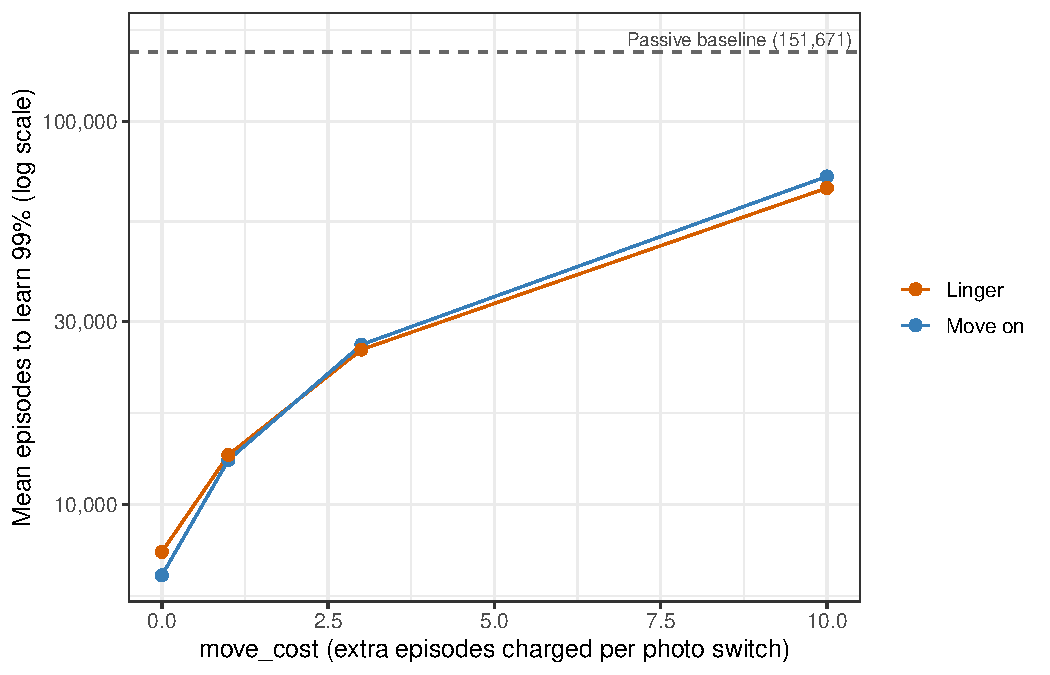
\includegraphics[width=0.8\linewidth]{flickr_linger_crossover.pdf}
\caption{\label{fig-flickr}
Mean episodes to learn 99\% of the vocabulary vs.\ \texttt{move\_cost}, active eliminative learner on Flickr8k captions. Moving on to a new photo wins when switching is cheap; lingering on the current photo overtakes it once switching costs more, with the crossover between \texttt{move\_cost}=1 and 3.}
\end{center}
\end{figure}

The linger-vs-move-on choice itself shows a genuine crossover rather than one policy dominating throughout. At \texttt{move\_cost} 0--1, always moving to a fresh photo wins: a new scene supplies more diverse elimination context than a second, independently-written description of the same one, so the extra information from a new scene outweighs the (zero or small) cost of obtaining it. Between \texttt{move\_cost} 1 and 3, the ranking flips, and lingering's advantage widens as switching gets more expensive--7\% faster than moving on at \texttt{move\_cost}=10. In other words, whether ``ask for more about what's already in view'' is the better strategy is not fixed; it depends on the relative cost of obtaining a new situation versus refining the current one, exactly the kind of parameter the companion paper's synthetic simulations, which never separated situation-content from situation-acquisition cost, could not have exposed.

This result should be read as a demonstration that the mechanism generalizes to real co-occurrence structure and that the linger-versus-move-on tradeoff is a real, locatable phenomenon, not as a claim about what value \texttt{move\_cost} actually takes for a child or caregiver in practice--we have no direct estimate of that value, and supplying one is a natural target for future work. It is also worth being explicit that Flickr8k captions are adult-crowdsourced descriptions of generic photographs, not child-directed speech or a child's own visual experience, so this study speaks to whether the mechanisms in the companion paper behave sensibly on naturalistic language statistics, not to developmental realism specifically.

\section{Study 2: A developmental passive-to-active trajectory}
\label{app-ramp}

Every active-learning condition in the companion paper holds the degree of autonomy fixed for the whole simulated lifetime of the learner--constantly active or constantly passive throughout; constant blends of the two are examined in Study 3 below. Real infants do not work this way: a newborn is carried from room to room with essentially no say over which scenes it experiences, and only gradually acquires the visual, postural, and locomotor control--head-turning, pointing, reaching, eventually crawling and walking--that lets it actively select what to attend to. This study asks whether that developmental trajectory itself, quite apart from its eventual endpoint, has consequences for how much of active selection's benefit a learner realizes.

\subsection{Motivation and setup}
The companion paper's completion-checkpoint analysis already implies an answer is possible: the active/passive gap widens over the course of learning (roughly 4-fold at 50\% completion, 9-fold at 90\%, 19-fold at 99\%, for the eliminative learner at $C=10$), meaning active selection's marginal value is low early--common words get learned quickly under either policy--and high late, when only rare stragglers remain. If a fixed ``active budget'' is worth more late than early, a learner who starts passive and becomes active over time should outperform a constant blend that spends the same budget evenly, and should do considerably better than a learner who front-loads the same budget into the early, low-value period.

We extended the eliminative learner with an optional \texttt{active\_prob\_fn}: a function of the episode count, re-evaluated every episode, in place of a constant \texttt{active\_prob}. We compare a forward, linear ramp from passive to active, $\text{active\_prob}(t) = \min(1, t/T)$, against its mirror image, a reverse ramp from active to passive, $\text{active\_prob}(t) = \max(0, 1-t/T)$--the reverse direction serving as a directional sanity check, since it spends an identical total ``active investment'' but places it exactly where the checkpoint analysis says it is worth least. Both are indexed by episode count rather than fraction of vocabulary learned, since real motor and attentional development runs on its own maturational clock and is not contingent on how much vocabulary a particular child happens to have acquired so far; this makes the ramp's timescale $T$ a free parameter, swept here (at $M=1{,}000$, $C=10$, $a=1$, 30 replications per condition) rather than fixed at a single guessed value.

\subsection{Results}
Table~\ref{tab-ramp} gives the fixed reference points--pure passive and active sampling, and constant blends at four intermediate autonomy levels--and Figure~\ref{fig-ramp} shows both ramp directions across seven timescales, $T \in \{1{,}000, 2{,}000, 3{,}000, 5{,}000, 8{,}000, 12{,}000, 20{,}000\}$ episodes.

\begin{table}[h]
\centering
\caption{\label{tab-ramp} Mean episodes to learn 99\% of a Zipfian ($a=1$), $M=1{,}000$-word vocabulary, eliminative learner, $C=10$: fixed reference points (no developmental trajectory).}
\begin{tabular}{lr}
\hline
Condition & Episodes \\
\hline
Passive (active\_prob=0)     & 91{,}963 \\
Constant blend, active\_prob=0.10 & 20{,}907 \\
Constant blend, active\_prob=0.25 & 12{,}527 \\
Constant blend, active\_prob=0.50 &  7{,}823 \\
Constant blend, active\_prob=0.75 &  5{,}888 \\
Active (active\_prob=1)      &  4{,}659 \\
\hline
\end{tabular}
\end{table}

\begin{figure}[h]
\begin{center}
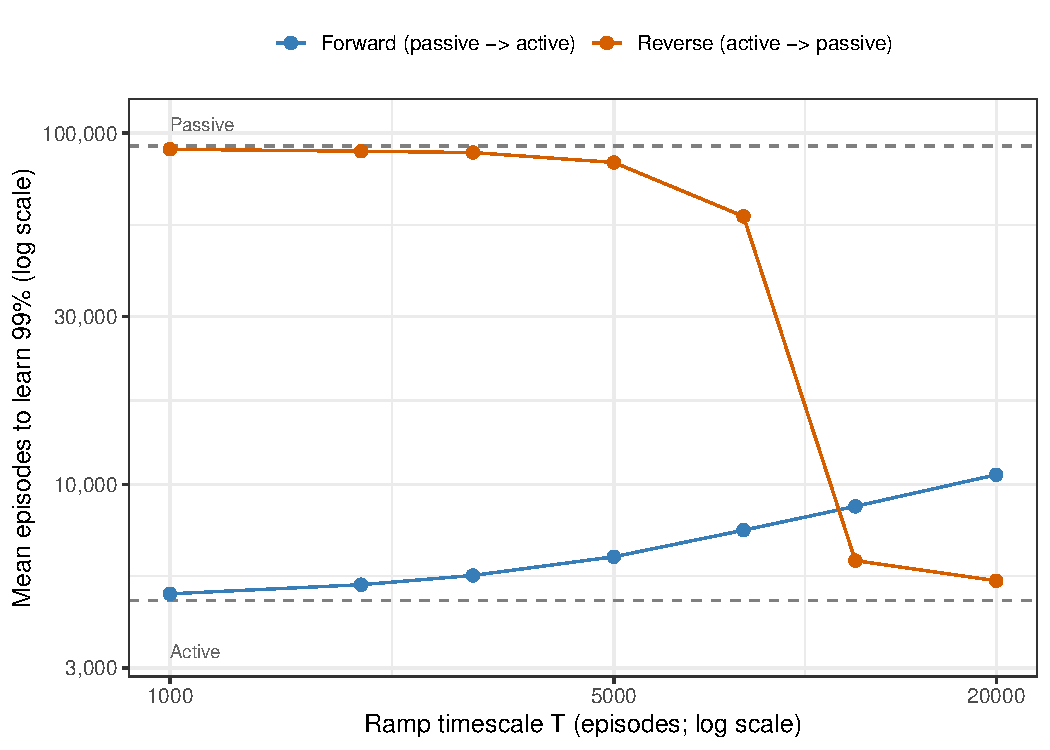
\includegraphics[width=0.8\linewidth]{active_ramp.pdf}
\caption{\label{fig-ramp}
Mean episodes to learn 99\% of the vocabulary vs.\ ramp timescale $T$, forward (passive-to-active) vs.\ reverse (active-to-passive) developmental trajectories. Dashed lines mark the pure passive and pure active reference points from Table~\ref{tab-ramp}.}
\end{center}
\end{figure}

The clearest single comparison is at the shortest timescale tested. A forward ramp with $T=1{,}000$--fully passive for the first 1,000 episodes, then linearly increasing to fully active--reaches 99\% in 4,874 episodes, within 4.6\% of pure active sampling (4,659). The reverse ramp at the identical $T=1{,}000$--fully active for the first 1,000 episodes, then decaying to fully passive--reaches 99\% in 89,961 episodes, statistically indistinguishable from pure passive sampling (91,963). Same timescale, same total quantity of active exposure, opposite placement in the learning trajectory: one recovers essentially all of active selection's benefit, the other essentially none of it.

Extending the sweep past the original three timescales reveals a further, unanticipated regularity. The forward ramp increases smoothly and monotonically with $T$, exactly as expected: more time spent passive before transitioning costs more, roughly in proportion to $T$ itself (4,874 at $T=1{,}000$ up to 10,643 at $T=20{,}000$). The reverse ramp, by contrast, does not decline smoothly--it stays close to the passive baseline through $T=8{,}000$ (57,934) and then falls sharply by $T=12{,}000$ (6,059), a roughly ten-fold drop between two adjacent timescales rather than a gradual one. We interpret this as follows: for large $T$, an active-heavy start completes the vocabulary quickly enough that the ramp never gets far into its decay before the learner is essentially done, so the process behaves like sustained high activity rather than a genuine transition to passivity. For small $T$, activity decays away well before the vocabulary is anywhere near complete, so nearly the entire (much longer) remaining run happens under passive-like conditions. The threshold falls close to pure active sampling's own completion time (4,659 episodes)--exactly where a fast, active-driven trajectory would either finish before the ramp bites (large $T$) or run headlong into a fully-decayed, passive-dominated remainder (small $T$)--which is a satisfying, if informal, confirmation that the mechanism we propose is the right one.

\subsection{Scope}
These results support a narrow but useful claim: a plausible developmental trajectory--little control early, more control later--is not merely ``a blend of the extremes'' with a worse average, and under the mechanism we model here, it need not sacrifice much of active selection's benefit relative to being fully active from birth, provided the transition happens on a fast-enough timescale relative to the vocabulary at hand. We make no claim about what timescale actually describes real infant development, nor have we tested ramp shapes other than linear, or mechanisms other than eliminative learning at a single $C$ and Zipf exponent; extending this analysis to the other learning mechanisms and to a data-driven estimate of the transition's real timescale--plausibly informed by egocentric video of infants' own visual experience as their motor repertoire develops--is a natural next step, not one we take here.

\section{Study 3: How much autonomy, and over what?}
\label{sec-modes}

Studies 1 and 2 ask how active selection is deployed across situations and across developmental time. A third question concerns the active learner itself. In the companion paper, an active learner is idealized in two ways: it exercises choice on every episode, and whenever it does, it can choose among the entire vocabulary, preferring any word it does not yet know. Real learners exercise control only some of the time; they choose among whatever happens to be available (the toys in the room, not every object they will ever name); and they may not simply prefer the least-known item, since infants preferentially attend to stimuli of intermediate familiarity \citep[the ``Goldilocks effect'';][]{Kidd:2012}. This study relaxes each idealization in turn.

\subsection{Setup}
We extended the eliminative learner's target selection in three ways. \textit{Partial autonomy}: each episode is active with probability $\text{active\_prob} \in \{0.25, 0.5, 0.75\}$ and passive otherwise, a constant blend of the kind used as the reference point in Study 2. \textit{Goldilocks targeting}: among not-yet-known words, the learner prefers those it has encountered about twice, weighting each by $\exp(-(n-2)^2/8)$ times its frequency, where $n$ is the number of times the word has been the target so far. \textit{Bounded choice}: on each active episode the learner may choose only among a choice set of $k \in \{100, 50, 20, 5\}$ words, drawn without replacement in proportion to frequency (so that commonly-encountered things are more likely to be at hand), preferring an unknown word within the set and making a passive draw from the set if it contains none.

We ran each condition, together with pure passive and fully active selection, in four settings for a Zipfian vocabulary of $M=1{,}000$ words: $C=10$ with random and with familiar context selection ($a=1$), and two settings at $C=100$. The companion paper shows that at $C=100$, $a=1$, the eliminative learner never completes with randomly-composed contexts, even under fully active selection, so there we use the two $C=100$ settings in which learning does complete: familiar context at $a=1$, and random context at $a=0.75$, the steepest skew at which random-context learning finished in every run. All conditions were simulated with the companion paper's fast reimplementation of the eliminative learner, which we validated for each of these target-selection rules against the reference implementation (200 replications per condition at $C=10$, 30 at $C=100$).

\subsection{Results}
Table~\ref{tab-modes} and Figure~\ref{fig-modes} report each condition's episodes to learn 99\% of the vocabulary relative to fully active selection in the same setting.

\begin{table}[h]
\centering
\caption{\label{tab-modes} Episodes to learn 99\% of an $M=1{,}000$-word Zipfian vocabulary, eliminative learner, relative to fully active selection in the same setting (first row: fully active episodes). Values above 1 are slower than fully active.}
\small
\begin{tabular}{lrrrr}
\hline
 & \multicolumn{2}{c}{$C=10$, $a=1$} & \multicolumn{1}{c}{$C=100$, $a=0.75$} & \multicolumn{1}{c}{$C=100$, $a=1$} \\
Condition & Random & Familiar & Random & Familiar \\
\hline
Fully active (episodes) & 4{,}692 & 3{,}132 & 628{,}691 & 16{,}060 \\
\hline
Passive & 19.0x & 14.2x & 10.6x & 26.6x \\
25\% active & 2.67x & 2.51x & 2.33x & 1.81x \\
50\% active & 1.67x & 1.63x & 1.58x & 1.34x \\
75\% active & 1.24x & 1.23x & 1.21x & 1.11x \\
Goldilocks & 1.00x & 1.04x & 1.00x & 0.56x \\
Choice set of 100 & 1.03x & 1.09x & 1.03x & 5.51x \\
Choice set of 50 & 1.13x & 1.15x & 1.09x & 8.01x \\
Choice set of 20 & 1.54x & 1.43x & 1.32x & 11.3x \\
Choice set of 5 & 4.15x & 3.32x & 2.78x & 10.4x \\
\hline
\end{tabular}
\end{table}

\begin{figure}[h]
\begin{center}
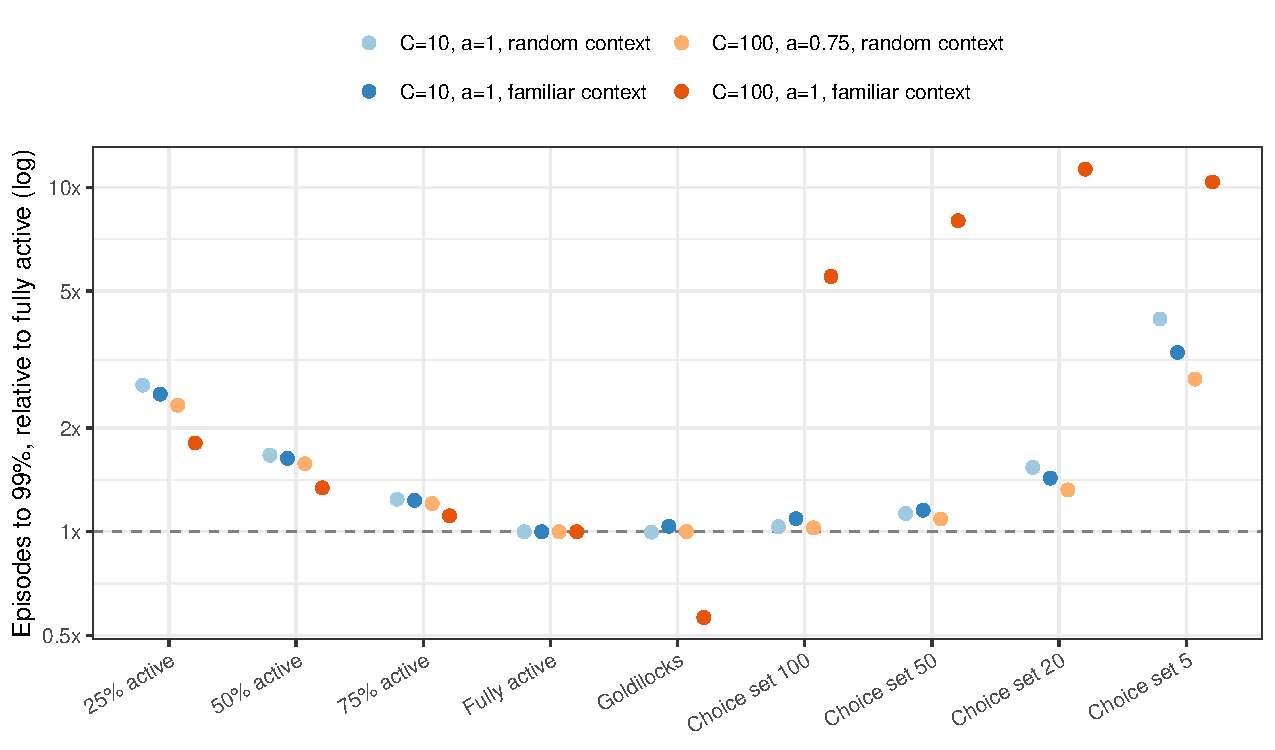
\includegraphics[width=\linewidth]{active_modes.pdf}
\caption{\label{fig-modes}
Episodes to learn 99\% of the vocabulary relative to fully active selection (log scale; dashed line = fully active), eliminative learner, for partial autonomy, Goldilocks targeting, and bounded choice sets, in four settings. Pure passive sampling (10.6--26.6x) is omitted for scale.}
\end{center}
\end{figure}

\textit{Partial autonomy shows steeply diminishing returns.} In every setting, a learner who is active on only a quarter of episodes already captures most of active selection's benefit: measured on a log scale, between two-thirds and four-fifths of the full passive-to-active speedup (e.g., at $C=10$ with random context, 7.1x of a possible 19.0x). Each further increment of autonomy buys less. This agrees with the constant blends in Study 2 (Table~\ref{tab-ramp}), and complements it: Study 2 shows that \textit{when} autonomy arrives matters a great deal, while this study shows that, once it has arrived, even occasional exercise of it goes a long way.

\textit{Goldilocks targeting matters in only one setting.} Preferring words encountered about twice makes no difference in three of the four settings (0.996--1.04x), but nearly halves learning time at $C=100$ with familiar context (0.56x).

\textit{The cost of bounded choice depends on the setting.} In three settings, restricting choice costs little until the choice set is small, and costs more the smaller it is (1.03--1.09x with 100 words to choose from, rising to 2.8--4.1x with 5). At $C=100$ with familiar context, the pattern is different: even a choice set of 100 makes learning 5.5 times slower, and the cost is not monotone in the size of the set (11.3x with 20 words, 10.4x with 5).

A diagnostic isolates the cause of this last pattern. Drawing the choice set uniformly rather than in proportion to frequency, and otherwise leaving everything unchanged, removes the cost almost entirely at $C=100$ with familiar context: 15,124 episodes with a uniform set of 100 words and 15,894 with 20, against 15,876 for unrestricted choice (30 replications each). The cost therefore comes not from restricting choice as such but from choice sets that over-represent frequent words: when the set is drawn by frequency and the target is then chosen from it by frequency again, a rare word's chance of being targeted scales roughly with the square of its frequency, and rare words are rarely targeted at all. Together with the Goldilocks result, this suggests that at $C=100$ with familiar context, learning is fastest when exposures are spread across the whole vocabulary, including its rare words.

\subsection{Mechanism: unseen words dilute the familiarity signal}
Why should spreading exposures matter, and only with familiar context at large $C$? Familiar-context selection weights each candidate distractor $r$ by $1/(n_r+1)$, where $n_r$ is the number of words that still hold $r$ as a possible meaning. A word that has never been the target of an episode has eliminated nothing, so it still holds every referent as a possible meaning, and each such unseen word adds the same amount to every referent's $n_r$. While many words are unseen, this shared count swamps the differences between referents, and familiar-context selection behaves almost like random selection. On this account, familiar context only starts to help once most words have been encountered at least once, and policies that concentrate targets on frequent words delay that point.

We tested this account in two ways, both at $C=100$, $a=1$ with familiar context (Table~\ref{tab-dilution}, Figure~\ref{fig-dilution}). First, we removed the dilution by computing each referent's familiarity from encountered words only, i.e.\ discounting the contribution of unseen words. If dilution is the mechanism, this should largely remove the differences between policies, and it does. The frequency-weighted choice set of 100 words goes from 5.7 times slower than unrestricted choice to 1.3 times; Goldilocks targeting goes from 0.57 to 0.93. At the 50\% checkpoint, the choice-set cost disappears entirely (5,547 episodes vs.\ 5,127 unrestricted, down from 84,671). What remains for small frequency-weighted choice sets (3.3x for 20 words) arises late in learning, and reflects the separate, direct problem that rare words are seldom in the choice set and so are seldom targeted. Removing the dilution also halves learning time for unrestricted active selection (15,770 to 7,803 episodes), while leaving passive sampling essentially unchanged (466,339 to 451,567), whose bottleneck is instead how rarely its rare words are targeted.

Second, we tracked each policy's trajectory under the original weighting. The frequency-weighted choice set leaves many words unencountered for a long time--634 after 10,000 episodes, against 63 for unrestricted choice and 34 for a uniform choice set--and throughout this period, 96--98\% of a target's remaining competing referents reappear among its distractors, escaping elimination, against 66--84\% for the other policies. Goldilocks targeting, which favors words encountered only once or twice, brings the number of unencountered words down fastest (33 after 5,000 episodes) and has the lowest competitor survival (about 50\%).

\begin{table}[h]
\centering
\caption{\label{tab-dilution} Episodes to learn 99\% of an $M=1{,}000$-word Zipfian ($a=1$) vocabulary at $C=100$ with familiar context, relative to unrestricted active selection under the same familiarity measure (30 replications per cell). ``All words'': the original familiarity measure, in which every unencountered word counts as still holding every referent; ``encountered words only'': that contribution removed.}
\small
\begin{tabular}{lrr}
\hline
 & \multicolumn{2}{c}{Familiarity computed from} \\
Condition & All words & Encountered words only \\
\hline
Unrestricted active (episodes) & 15{,}770 & 7{,}803 \\
\hline
Choice set of 100, frequency-weighted & 5.66x & 1.34x \\
Choice set of 20, frequency-weighted & 11.2x & 3.32x \\
Choice set of 100, uniform & 0.96x & 1.01x \\
Goldilocks & 0.57x & 0.93x \\
Passive & 29.6x & 57.9x \\
\hline
\end{tabular}
\end{table}

\begin{figure}[h]
\begin{center}
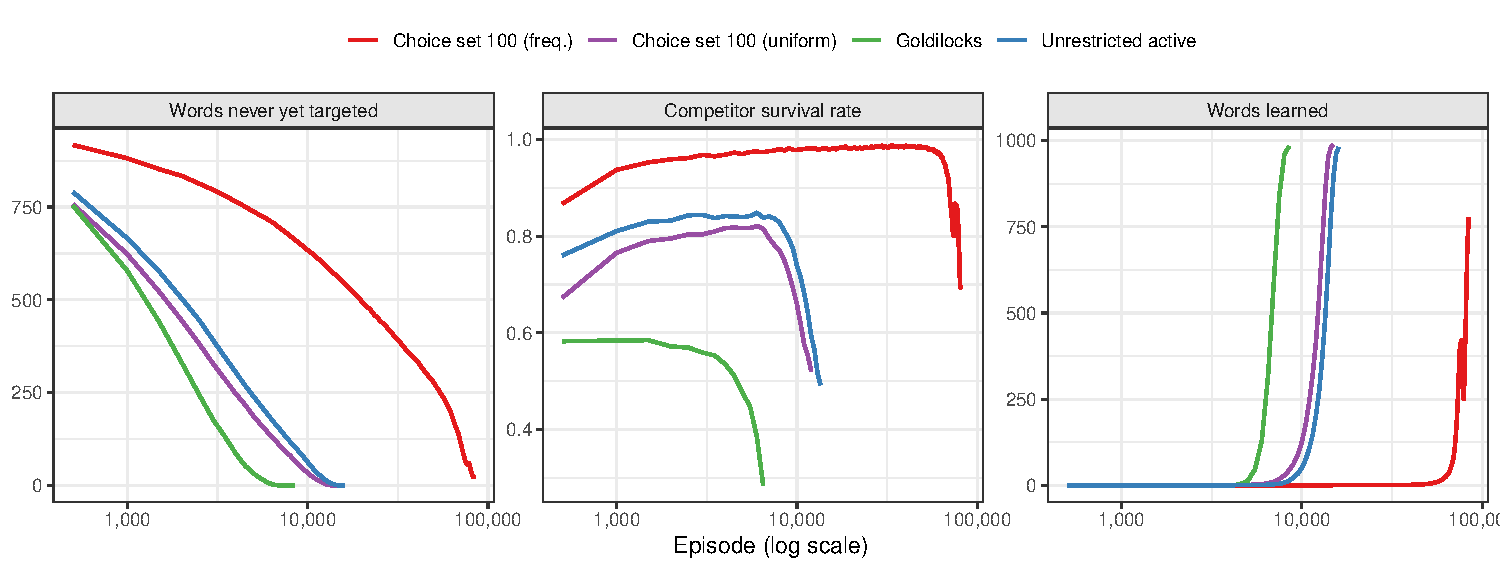
\includegraphics[width=\linewidth]{familiar_dilution.pdf}
\caption{\label{fig-dilution}
Trajectories under the original familiarity measure, $C=100$, $a=1$, familiar context (means of 10 runs). Left: words never yet targeted. Middle: competitor survival, the share of the target's remaining competing referents that reappear among its distractors and so escape elimination, shown until half the vocabulary is learned. Right: words learned. The frequency-weighted choice set leaves many words unencountered for longer, and while it does, familiar-context selection barely reduces competitor survival.}
\end{center}
\end{figure}

Why only at large $C$? At $C=10$ elimination is fast even with random distractors, so familiar-context selection adds relatively little (the companion paper reports a 2-fold benefit at $C=10$, against a difference between learning and not learning at all at $C=100$), and a policy that delays its benefit loses correspondingly little.

These tests also suggest a modeling point. The dilution arises from treating a never-encountered word as ``still considering every referent'', which is the natural bookkeeping for an eliminative learner, but not the only plausible one: a learner that simply ignores words it has not yet heard when judging how familiar an object is learns twice as fast under unrestricted active selection, and is far less sensitive to how its choice set is composed.

\subsection{Scope}
Two conclusions seem robust across the settings we tested: partial autonomy has steeply diminishing returns, and most of active selection's benefit survives a learner who exercises it only occasionally. The results for Goldilocks targeting and bounded choice are more conditional. Their size, and at $C=100$ with familiar context their direction relative to other settings, depends on context size and on whether distractors are controlled, and at least for bounded choice, on what the available choice set contains rather than merely how large it is. If children's accessible objects are, like the objects they encounter generally, dominated by common ones, the composition of what is at hand may matter as much as the freedom to choose among it. We have tested only the eliminative mechanism, four settings, and frequency-weighted or uniform choice sets; how real choice sets are composed, and how large they are, are empirical questions we do not address.

\section{Discussion (TODO)}
Not yet written. Should connect Studies 1--3 under the shared theme sketched in the Introduction bullets, discuss the foraging-theory and infant-motor-development literatures (and, for Study 3, the literature on curiosity and intermediate-familiarity preferences), and be explicit about what would be needed to strengthen the "unifying claim" from thematic to mechanistic.

\bibliographystyle{apacite}
\setlength{\bibleftmargin}{.125in}
\setlength{\bibindent}{-\bibleftmargin}
\bibliography{../paper/corpusXSL_refs}

\end{document}
